%======================================================================
\section*{Task 5. PINN for the Silverbox oscillator}
%======================================================================
\textbf{Code:} \url{\repourl}, folder \texttt{task5\_pinn\_silverbox/}\\
(\texttt{silverbox\_pinn.py}: data, network, RK4, training, metric; \texttt{sweep.py}: all runs below;
\texttt{make\_figures.py}: plots and this section's numbers). PyTorch, float64.

\subsection*{Data}
\texttt{SNLS80mV.mat}, $u=$ \texttt{V1}, $y=$ \texttt{V2}, slice $[42650:46746]$ (4096 samples), each signal centred by its mean
on the excerpt ($\bar u=6.66$\,mV, $\bar y=1.32$\,mV). Train: samples $0$--$3071$ (5.03\,s); test: $3072$--$4095$ (1.68\,s).
The output spectrum peaks at 70.0\,Hz, the input band ends at 200\,Hz, the RMS of the test output is $60.49$\,mV (the zero
predictor). One property of this split decides the design: \textbf{the test segment reaches $|y|=0.205$\,V while the training
record never exceeds $0.174$\,V}, so on the largest test peak the force has to be extrapolated exactly where the cubic term is
strongest.

\subsection*{Model}
Equation (1), $\ddot y+a\dot y+by+cy^3=g\,u(t)$, in state form with $v=\dot y$:
\[
\dot y=v,\qquad \dot v=\alpha_\theta(y,v,u),
\]
where $\alpha_\theta$ is a fully connected network. \emph{Scaling:} the inputs are $(y/\sigma_y,\ v/\sigma_v,\ u/\sigma_u)$ and
the raw output is multiplied by $\sigma_a$, the standard deviations on the training record ($\sigma_y=53.0$\,mV,
$\sigma_v=22.4$\,V/s, $\sigma_u=22.0$\,mV, $\sigma_a=1.04\cdot10^{4}$\,V/s$^2$), so every input and the target are $O(1)$.
Architectures tried: A1 $2\times32$ tanh, A2 $2\times64$ tanh, A3 $3\times64$ tanh, A4 $2\times64$ SiLU (all with a linear output).

\emph{Integrator:} classical RK4 at $\Delta t=1/f_s$, driven by the measured input: stage 1 uses $u_k$, stages 2--3 use
$u(t_k+\Delta t/2)$, stage 4 uses $u_{k+1}$. The half-sample values come from a 16-tap Hann-windowed sinc interpolator of the
measured $u$ (the input is a multisine up to 200\,Hz, where the plain average $(u_k+u_{k+1})/2$ would keep only
$\cos(\pi\cdot200/610)\approx0.51$ of the amplitude); only $u$ is used, which is known on the whole excerpt.

\subsection*{Training (only the 3072 training samples enter any loss)}
\begin{enumerate}[leftmargin=*,itemsep=1pt]
\item \textbf{Stage A, identify the equation.} The four coefficients of (1) are first fitted to the training record: least
squares on finite-difference derivatives as the start, then the same rollout loss as in stage C (Adam, lr $3\cdot10^{-3}$,
600 steps, rollout 256). This is run \texttt{R\_duffing} in the table; it gives
$a=\identa$\,s$^{-1}$, $b=\identb$\,s$^{-2}$ ($f_0=\sqrt b/2\pi=68.4$\,Hz), $c=\identc$\,V$^{-2}$s$^{-2}$, $g=\identg$\,s$^{-2}$.
At $|y|=0.2$\,V the cubic force is $cy^2/b=16\%$ of the linear force.
\item \textbf{Stage B, residual pre-fit (collocation on the data).} 500 Adam steps on
$\|\ddot y_\text{FD}-\alpha_\theta(y,\dot y_\text{FD},u)\|^2/\sigma_a^2$ with 4th-order central differences. It gives the network
the right sign and size of the restoring force before any rollout.
\item \textbf{Stage C, rollout training + PINN residual.} Each step draws 32 windows at random starts in the training record,
starts each at the measured $y$ and the 4th-order finite-difference velocity, integrates with RK4 and penalises
\[
\mathcal L=\frac{1}{\sigma_y^2}\,\overline{(\hat y-y)^2}\;+\;\lambda_\text{phys}\,\frac{1}{\sigma_a^2}\,
\overline{\big(\alpha_\theta(\tilde y,\tilde v,\tilde u)+a\tilde v+b\tilde y+c\tilde y^3-g\tilde u\big)^2},
\]
the second term on 512 collocation points per step drawn uniformly from a box $1.5\times$ the training maxima of $|y|,|v|,|u|$
(it reaches $|y|=0.26$\,V, past the test peak). $a,b,c,g$ are the stage-A values, held fixed: they are not weights of the network,
and only the network is integrated at test time. The rollout length grows geometrically from 16 to the final length over the
first 40\% of the steps; cosine learning-rate decay to 5\%, gradient-norm clip 1. Every 100 steps the free run of the
training record is computed, and the weights with the lowest \emph{training} free-run RMSE are kept for that run.
\end{enumerate}

\subsection*{Metric}
After the weights are fixed: one free run of all 4096 samples from $y_0$ and the one-sided finite difference
$v_0=(-3y_0+4y_1-y_2)/2\Delta t$, RK4 through the training samples and on through the test samples with the same state, reading
$u$ only. RMSE on samples $3072$--$4095$ (test) and on $0$--$3071$ (train).

\subsection*{Results}
\begin{center}
\fbox{\begin{minipage}{0.9\linewidth}\centering
Kept version: \textbf{\keptnametex}\ \ (\keptarch, \keptparams\ weights)\\[2pt]
\textbf{free-run RMSE on the test record (1024 samples): \kepttest\,mV}\\[1pt]
free-run RMSE on the training record (3072 samples): \kepttrain\,mV\\[1pt]
zero-prediction baseline on the test record: 60.49\,mV
\end{minipage}}
\end{center}
\keptsettings

All runs (sorted by name; highlighted: kept). ``train''/``test'' are the free-run RMSEs of the metric, in mV.
A$k$\_h$j$ = architecture $k$ with training setting $j$; L\_* = ablation of the physics loss on A2\_h2; R\_* = references that are
not networks (4 coefficients of eq.~(1), trained by the same rollout loss; R\_linear has $c=0$).
{\footnotesize\setlength{\tabcolsep}{4pt}\sweeptable}

\keptdiscussion

\begin{figure}[H]\centering
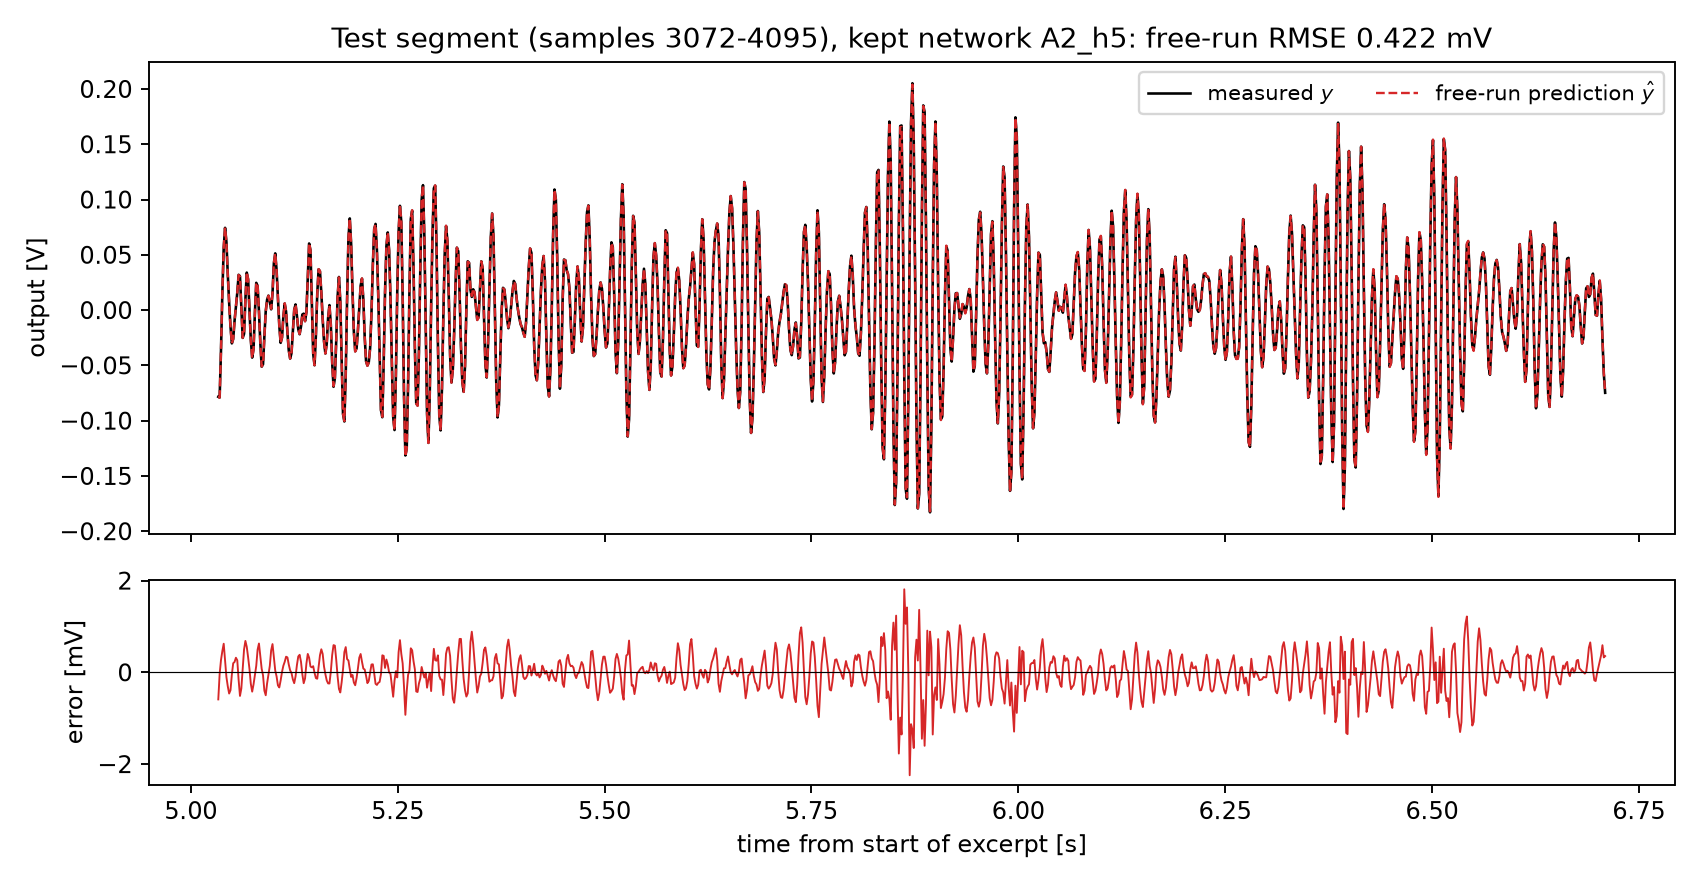
\includegraphics[width=\linewidth]{../task5_pinn_silverbox/figures/test_segment.png}
\caption{Measured output and free-run prediction of the kept network on the test segment, and the error.}
\end{figure}
\begin{figure}[H]\centering
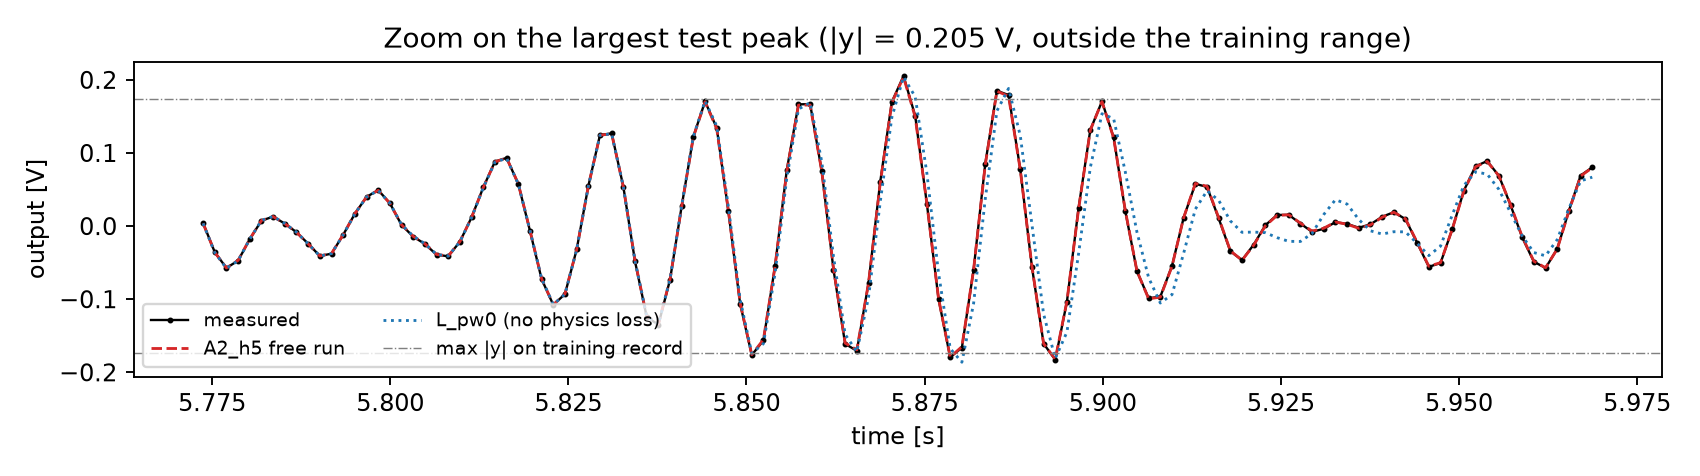
\includegraphics[width=\linewidth]{../task5_pinn_silverbox/figures/test_peak_zoom.png}
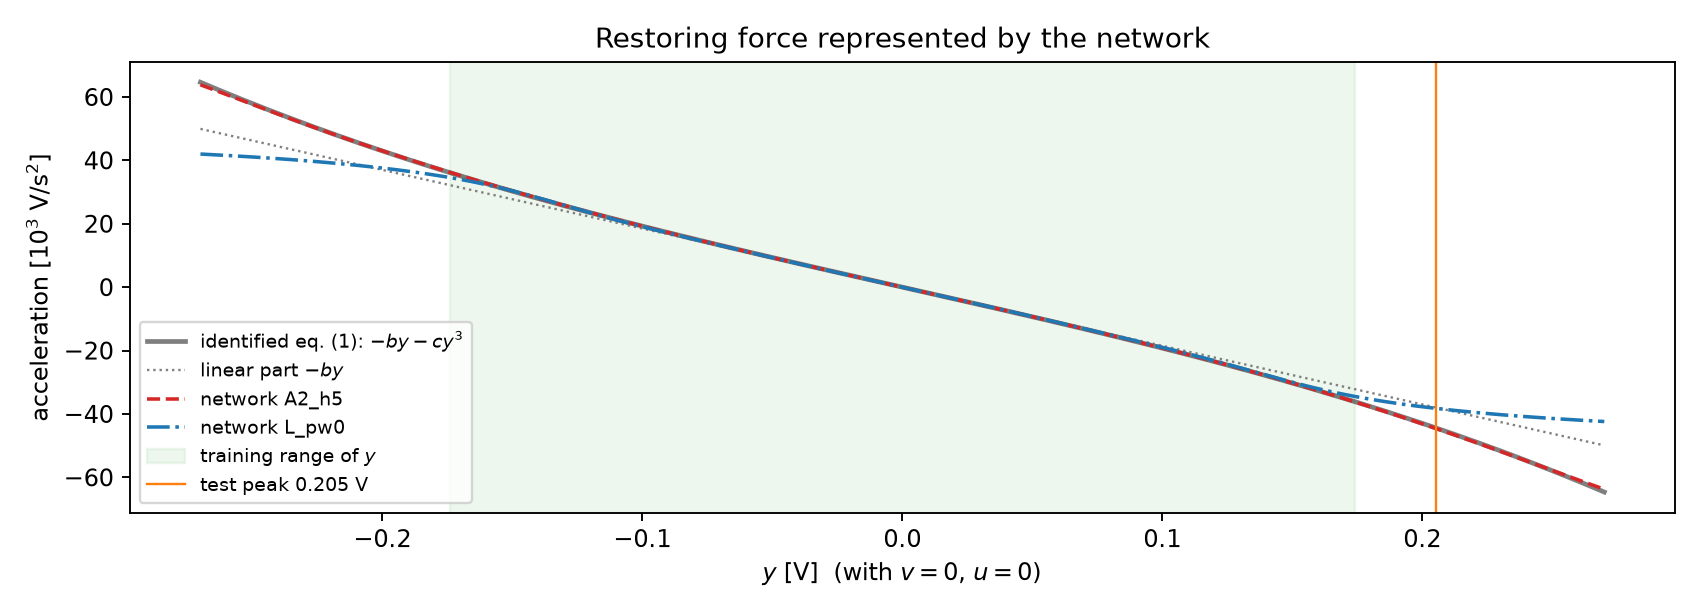
\includegraphics[width=\linewidth]{../task5_pinn_silverbox/figures/force_curve.png}
\caption{Top: the largest test peak, outside the training amplitude range, with and without the physics loss.
Bottom: the restoring force $\alpha_\theta(y,0,0)$; the network trained without the physics loss under-stiffens past the training range.}
\end{figure}

\paragraph{Physics read-out of the kept network.} Projecting $\alpha_\theta$ on the training states onto
$\{-v,-y,-y^3,u\}$ by least squares gives $a=\reada$, $b=\readb$ ($f_0=\readfzero$\,Hz), $c=\readc$, $g=\readg$ with
$R^2=\readrsq$: the network represents a Duffing-like force, in line with the stage-A identification.

%======================================================================
\section*{Task 6. Agentic system}
%======================================================================
\textbf{Code:} \url{\repourl}, folder \texttt{task6\_agentic\_system/}.\\
Files: \texttt{agents.py} (state, prompts, nodes, graph),
\texttt{coding\_tool.py}, \texttt{run\_task5.py} (gives the system Task 5), \texttt{render\_transcript.py},
\texttt{tests/offline\_smoke\_test.py}. LangGraph, LangChain; the model behind the roles is chosen with \texttt{--model}.
The run below used Claude Sonnet 5.5 through the Claude Code CLI (\texttt{--model claude-cli:claude-sonnet-5-5},
\texttt{claude\_cli.py}), with the CLI's own tools switched off: decisions are its structured output, and the executor's
coding-tool calls are requested as structured output and run by the executor node.

\begin{center}
\begin{tikzpicture}[>=Stealth, node distance=1.6cm,
  box/.style={draw,thick,rounded corners,minimum width=26mm,minimum height=9mm,align=center,font=\small}]
  \node[box,fill=blue!8] (o) {orchestrator\\\scriptsize decision = model call};
  \node[box,left=2.4cm of o] (s) {START\\\scriptsize user turn};
  \node[box,right=2.4cm of o] (e) {END};
  \node[box,fill=green!8,below left=1.6cm and 0.4cm of o] (sc) {scientist\\\scriptsize theory + plan};
  \node[box,fill=green!8,below=1.6cm of o] (g) {general\\\scriptsize side questions};
  \node[box,fill=orange!12,below right=1.6cm and 0.4cm of o] (ex) {executor\\\scriptsize coding tool};
  \draw[->,thick] (s) -- (o);
  \draw[->,thick] (o) -- node[above,font=\scriptsize]{finish} (e);
  \draw[->,thick] (o.south west) to[bend right=15] (sc.north);
  \draw[->,thick] (sc.north east) to[bend right=15] (o.240);
  \draw[->,thick] (o.265) -- (g.95);
  \draw[->,thick] (g.85) -- (o.275);
  \draw[->,thick] (o.south east) to[bend left=15] (ex.north);
  \draw[->,thick] (ex.north west) to[bend left=15] (o.300);
  \node[font=\scriptsize,align=left,right=0.3cm of ex] {write \texttt{*.py}\\run (300\,s limit)\\$\to$ exit code, stdout, stderr};
\end{tikzpicture}
\end{center}

\paragraph{State.} The state of the \texttt{StateGraph} is the dialogue: a list of turns, each
\texttt{\{role, content, meta\}} (role name, the text it said, and machine-readable fields such as the decision or the tool
record), merged with \texttt{operator.add}, so every node reads all earlier turns, including what the other agents wrote, and
appends exactly one turn. Routing, the decision count and the finish check are all derived from the dialogue itself.

\paragraph{Edges.} \texttt{START}$\to$orchestrator; a conditional edge from the orchestrator to scientist, general, executor
or \texttt{END}, chosen by the orchestrator's decision; an edge back from each specialist to the orchestrator.

\paragraph{Orchestrator.} A model call with structured output \texttt{Decision(next\_role, instruction, reason)}, where
\texttt{next\_role} $\in\{$scientist, general, executor, finish$\}$. It sees the whole dialogue plus a status line (decision
$k$ of 8, whether a verified RMSE exists). It has no tool and its prompt forbids theory and code. Rules enforced in code:
at most 8 decisions; \texttt{finish} is accepted only if some executor turn holds a \texttt{TEST\_RMSE} parsed from the standard
output of a script that ran with exit code 0 --- otherwise the model is asked once more with the reason, and a second
\texttt{finish} is routed to the executor.

\paragraph{Scientist / general agent.} Model calls without tools. The scientist writes the equation, the network, the state
equation, the training, the free-run test and a numbered implementation list, and may not quote a number that no executor turn
printed. The general agent answers high-level side questions (what a record is, what a term or an error means) and writes no plan.

\paragraph{Executor and the coding tool.} The only role bound to the tool \texttt{coding\_tool(action, filename, code)}:
\texttt{write} creates a \emph{new} \texttt{.py} file in the run's working directory (existing names are refused, so every
implementation and every repair is a new file); \texttt{run} executes it with a 300\,s limit and returns exit code, stdout and
stderr. One write and one run per executor turn; the node appends a tool record (files, exit codes, the parsed
\texttt{TEST\_RMSE}/\texttt{TRAIN\_RMSE} marked VERIFIED, or the stderr tail with the traceback). A later executor turn sees
the previous script and can repair it; the plan stays the scientist's.

\subsection*{Validation run on Task 5}
Model behind every role: \texttt{claude-cli:claude-sonnet-5-5}. Turns: 6; orchestrator decisions: 3.

\textbf{Free-run error printed by the script that ran} (\texttt{silverbox\_pinn.py}): test RMSE $= 0.00100889$\,V, train RMSE $= 0.00144579$\,V.

\begin{longtable}{@{}r l p{0.72\linewidth}@{}}
\toprule \# & role & what it did\\ \midrule \endhead
1 & user & Please solve the following task with your team and report the verified free-run errors. Task 5. PINN (Physics Informed Neural Network) for the Silv...\\
2 & orchestrator & -\textgreater{} scientist: A plan must be written by the scientist before any code can be executed.\\
3 & scientist & \# Plan for Task 5: Silverbox PINN No numbers have been measured yet. Every size below is an expectation from the problem statement, not a result. \#...\\
4 & orchestrator & -\textgreater{} executor: The plan is complete, so it must now be coded and run to obtain verified RMSE values.\\
5 & executor & write silverbox\_pinn.py: ok run silverbox\_pinn.py: exit code 0, 210.0 s VERIFIED printed by the script: TEST\_RMSE=0.0010088887947707441, TRAIN\_RMSE=0.0014457...\\
6 & orchestrator & -\textgreater{} finish: A VERIFIED executor result with both TRAIN\_RMSE and TEST\_RMSE exists, so the run can be finished.\\
\bottomrule
\end{longtable}
\begin{figure}[H]\centering
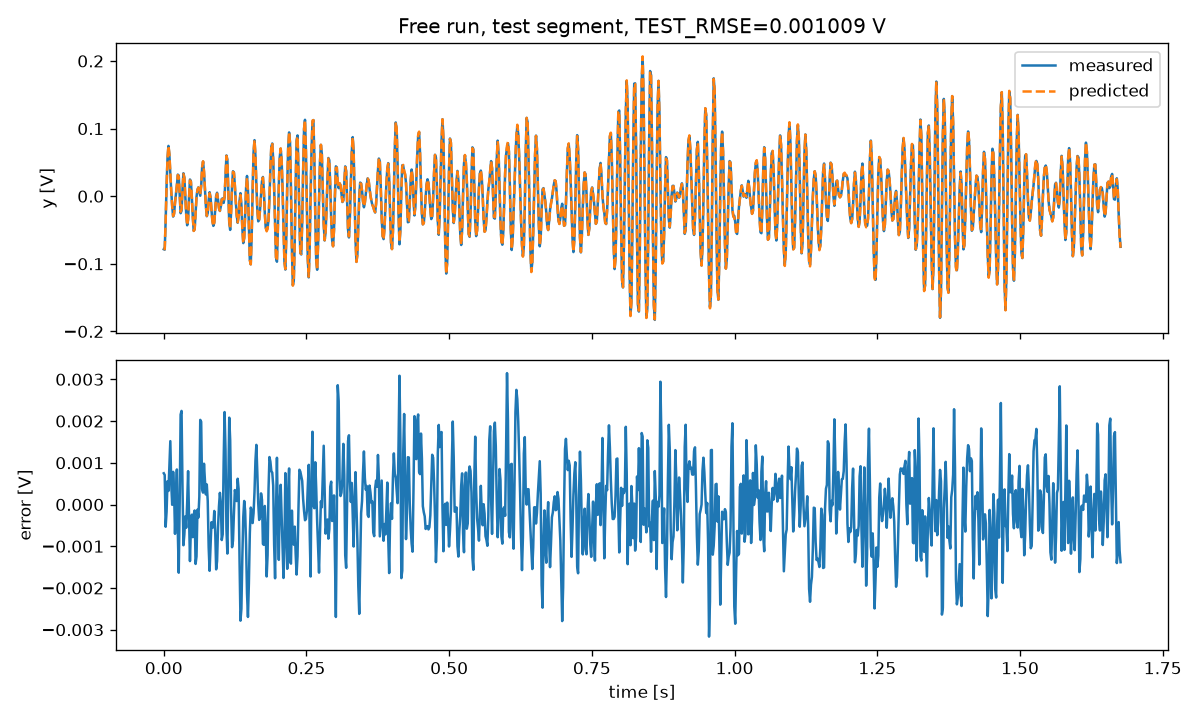
\includegraphics[width=0.85\linewidth]{../task6_agentic_system/runs/20261014-001143/work/test_segment.png}
\caption{The plot saved by the agents' script: measured output and free-run prediction on the test segment.}
\end{figure}

\paragraph{Transcript (abridged).}
\noindent\textbf{Turn 1 --- user}
\begin{lstlisting}
Please solve the following task with your team and report the verified free-run errors....
[the full Task 5 statement follows: task6_agentic_system/task5_statement.md]
\end{lstlisting}
\noindent\textbf{Turn 2 --- orchestrator}
\begin{lstlisting}
Decision 1/8 -> scientist
Instruction: Write the complete, code-ready plan for Task 5 (Silverbox PINN). Include: data loading from SNLS80mV.mat (V1=u, V2=y), slice [42650:46746], mean-centering, split 3072 train / 1024 test, dt=1/610.35. Network alpha_theta(y,v,u) with chosen depth/widths/activation and input/output scaling, optionally physics-informed initialization from eq. (1) (y''=-a v - b y - c y^3 + g u) with learnable a,b,c,g as a residual/prior (b ~ (2*pi*70)^2, a few tens). RK4 integration with u held/interpolated between samples (specify, e.g. midpoint u average), training scheme (multiple shooting over short windows, curriculum on window length, Adam then maybe LBFGS, learning rates, epochs), keeping total runtime under 5 minutes on CPU. Then the final free run: initial state from the first sample with finite-difference velocity, integrate through train into test without reading test y, print TRAIN_RMSE and TEST_RMSE, and save a plot of measured vs predicted on the test segment. Give a numbered list of steps specific enough to code.
Reason: A plan must be written by the scientist before any code can be executed.
\end{lstlisting}
\noindent\textbf{Turn 3 --- scientist}
\begin{lstlisting}
# Plan for Task 5: Silverbox PINN

No numbers have been measured yet. Every size below is an expectation from the problem statement, not a result.

## 1. Differential equation and coefficients

y'' + a y' + b y + c y^3 = g u(t), with y and u the mean-centered signals.

| Coef | Meaning | Expected size / initial value |
|---|---|---|
| a | damping, 1/s | tens, about 20-40 |
| b | linear stiffness, 1/s^2 | (2pi*70)^2 ~ 1.9e5 |
| c | cubic stiffness, 1/(V^2*s^2) | cy^2 ~ 0.1-0.3*b at |y| = 0.2, so c ~ 5e5-1.5e6 |
| g | input gain, V/(V*s^2) | order 1e4 (from y ~ g*u/(a*omega) at resonance); fix it by regression |

- a, b, c and g are four learnable scalars of the physics prior. They are not network weights.
- Initialize them by least squares on the training record (step 4), then refine them by shooting.
- The RK4 step at 70 Hz has omega*dt ~ 0.72, so the integrator carries phase and damping error of its own. Training and testing use the same integrator, so the fitted b and a will absorb this. This is intended and should not be "corrected".

## 2. Network

Acceleration: alpha_theta(y,v,u) = -a v - b y - c y^3 + g u + S_alpha * N_theta(y/S_y, v/S_v, u/S_u)

- **Scales** (computed from the training record only):
  - S_y = std(y_train)
  - S_v = omega?*S_y with omega? = 2pi*70
  - S_u = std(u_train)
  - S_alpha = omega?^2*S_y
- **MLP N_theta:** 3 -> 32 -> 32 -> 1, tanh activation, flo
[... abridged ...]
 after that run.

## Revision rules, if the first results are poor

- Keep eq. (1) and the free-run test unchanged.
- Diagnose from the train free-run error and the loss history, not from the test error.
- The first levers are a longer L in stage 3, 2 substeps per sample, a lower ?, and a larger network (64 units).
- If the rollout diverges, lower the learning rate and raise ?.
\end{lstlisting}
\noindent\textbf{Turn 4 --- orchestrator}
\begin{lstlisting}
Decision 2/8 -> executor
Instruction: Implement the scientist's latest plan (Silverbox PINN) in a new Python file and run it (5-minute limit). Follow the numbered steps exactly: load SNLS80mV.mat, slice [42650:46746], center, 3072/1024 split, least-squares init of a,b,c,g, physics-prior + zero-init residual MLP (3-32-32-1 tanh, float64), RK4 with midpoint u, multiple-shooting stages 0-3 (optional 4) with wall-clock guards, then one free run from sample 0 through train into test reading only u. Save the plot of measured vs predicted on the test segment to test_segment.png. Print the final a,b,c,g, and as the last two lines TRAIN_RMSE=<float> and TEST_RMSE=<float>. Return the printed output verbatim, or the full traceback if it fails.
Reason: The plan is complete, so it must now be coded and run to obtain verified RMSE values.
\end{lstlisting}
\noindent\textbf{Turn 5 --- executor}
\begin{lstlisting}
File: silverbox_pinn.py. Exit code: 0. Runtime was 207.6 s, inside the 5-minute limit. The plot was saved as test_segment.png.

Printed RMSE lines, exactly as printed:
TRAIN_RMSE=0.0014457934186479073
TEST_RMSE=0.0010088887947707441

Other printed values:
- Least-squares init: a=39.6, b=1.760e5, c=5.749e5, g=1.600e5.
- Final fitted values: a=41.19, b=1.848e5, c=7.4768e5, g=1.9608e5.
- Maximum |?| of the free run was 0.2068.
- The zero-predictor test RMSE was 0.0605.
- Training stage S3 hit its time budget at iteration 109 of 150.
- Stage 4 stopped after 8 iterations, at the 30 s budget.
- stderr held only a harmless PyTorch UserWarning about converting a tensor that requires grad to a float.

The free run started at sample 0 and carried its state through the train/test boundary. It read only u after the first sample.

[tool record]
write silverbox_pinn.py: ok
run silverbox_pinn.py: exit code 0, 210.0 s
VERIFIED printed by the script: TEST_RMSE=0.0010088887947707441, TRAIN_RMSE=0.0014457934186479073
\end{lstlisting}
\noindent\textbf{Turn 6 --- orchestrator}
\begin{lstlisting}
Decision 3/8 -> finish
Instruction: The Silverbox PINN ran and the script printed the free-run errors. The script is silverbox_pinn.py and the plot is test_segment.png.

Verified results, exactly as printed:
- TRAIN_RMSE=0.0014457934186479073
- TEST_RMSE=0.0010088887947707441

For scale, predicting zero scores 0.0605 V RMSE on the test segment, so the model is much better than the baseline.

Method:
- The model is eq. (1) as a physics prior with learnable a, b, c and g, plus a residual 3-32-32-1 tanh network whose last layer starts at zero.
- It was integrated with RK4 and trained by multiple shooting.
- The free run started at sample 0 with a finite-difference velocity. It carried the state through the train/test boundary and read only u after the first sample.

Fitted coefficients:
- Least-squares initialization: a=39.6, b=1.760e5, c=5.749e5, g=1.600e5.
- Final: a=41.19, b=1.848e5, c=7.4768e5, g=1.9608e5.

Other notes:
- The maximum |?| of the free run was 0.2068.
- The run took about 208 s.
- The last stage-3 and stage-4 runs stopped at their time budgets (iteration 109 of 150 and 8 iterations).
- stderr held only a harmless PyTorch UserWarning.
Reason: A VERIFIED executor result with both TRAIN_RMSE and TEST_RMSE exists, so the run can be finished.
\end{lstlisting}

